\chapter{High-Level and Low-Level Design}
\label{ch:design}
This chapter presents the design of FaceCon, from the overall architecture down to the classes, modules, and interface contracts that implement it. The design realizes the methodology of the previous chapter and keeps the pipeline stages modular, so that any stage can be developed, tested, or replaced independently and so that simple and complex models share common data and decode interfaces. Throughout the chapter it is important to keep three ideas distinct: the system (software) architecture, which is how the code and its components are organized; the machine-learning model architecture, which is the internal structure of a particular predictor such as an MLP or a transformer; and the modelling strategy, which is the baselines first progression described in Chapter~\ref{ch:method}. This chapter concerns the first of these, and refers to the other two only where the software must accommodate them.

\section{System Overview}
FaceCon is a layered, modular system. A thin interface layer exposes configuration-driven tools for the researcher-developer and evaluator, together with a lightweight local web demonstrator. Beneath it, a processing layer contains the pipeline modules for genotype QC and SNP selection, scan to FLAME fitting, subject matching and splitting, model training, and evaluation. A model layer holds the interchangeable shape predictors (mean-face, demographic, ridge, MLP, and optional advanced models) together with the shared FLAME decoder, and a parallel appearance component that integrates the established HIrisPlex-S predictor and renders its eye, hair, and skin colour outputs onto the decoded face. A data layer persists genotypes, registered meshes, FLAME parameters, splits, checkpoints, and results. This separation lets the scientific logic, the model definitions, and the storage evolve independently, and it keeps the demonstrator a thin client over the trained shape models and the integrated appearance predictor.

\section{Design Considerations}
This section records the assumptions, constraints, and guiding goals that shape the design before the architecture is presented, together with the development method followed. They are stated first because they explain choices that might otherwise look arbitrary, such as why the system stores files rather than a database, why every model sits behind one interface, and why the simplest adequate model is always preferred.

\subsection{Assumptions and Dependencies}
FaceCon assumes access to the required FLAME model files, genotype-processing tools, deep learning libraries, and 3D mesh utilities. It also depends on approved access to the 3DFN genotype and facial data, which must be stored and processed according to the applicable data-use agreement. The system assumes a consistent FLAME topology for facial representation. The main pipeline is intended for technical users, while the final demonstrator is designed so that evaluators can view and compare predictions without needing knowledge of the underlying implementation.

\subsection{General Constraints}
The design must respect privacy constraints, so that no raw individual-level data appears in released artifacts. It must satisfy reproducibility constraints, so that all runs are configuration- and seed-driven, and scientific constraints, so that splits are strictly subject-level with no leakage. It must also avoid machine-specific hard-coded paths, a defect explicitly identified in prior work.

\subsection{Goals and Guidelines}
The design follows the ``keep it simple'' principle. The smallest model that fits the data is preferred, because the paired-sample size is modest and over-large models would overfit and obscure the scientific question. Clarity and reproducibility are valued over architectural novelty.

\subsection{Development Methods}
Development is incremental. Each module is built and unit-tested against synthetic data first, so the full pipeline is runnable end-to-end before real data access is finalized, and it is then validated on real data as that data becomes available. Interchangeable data loaders for synthetic and real data share one interface, so that experiments can be developed before approval completes.

\section{System Architecture}
Figure~\ref{fig:arch} shows the layered architecture. Control flows downward from the interface layer, which issues configuration-driven commands. The processing layer orchestrates the pipeline, the model layer performs training and inference, and the data layer persists every artifact. The rationale for this decomposition is that the expensive, one-time data preparation is cleanly separated from the frequently-repeated model experimentation, and that a shared decode and evaluation interface lets every model, from mean-face to advanced, be compared on equal terms.

\begin{figure}[!ht]
\centering
\begin{tikzpicture}[node distance=0.5cm,every node/.style={font=\footnotesize}]
\tikzstyle{lay}=[draw,rounded corners,minimum width=12.5cm,minimum height=0.95cm,align=center]
\node[lay,fill=gray!10](i){Interface Layer --- configuration-driven CLI (developer, evaluator) $\vert$ local web demonstrator};
\node[lay,below=0.8cm of i,fill=blue!4,minimum height=1.5cm](p){};
\node[font=\bfseries] at ([yshift=0.5cm]p.center){Processing Layer};
\node[draw,fill=white,font=\scriptsize] at ([yshift=-0.1cm,xshift=-4.8cm]p.center){QC + SNP};
\node[draw,fill=white,font=\scriptsize] at ([yshift=-0.1cm,xshift=-2.2cm]p.center){FLAME fit};
\node[draw,fill=white,font=\scriptsize] at ([yshift=-0.1cm,xshift=0.3cm]p.center){Matching};
\node[draw,fill=white,font=\scriptsize] at ([yshift=-0.1cm,xshift=2.6cm]p.center){Training};
\node[draw,fill=white,font=\scriptsize] at ([yshift=-0.1cm,xshift=5.0cm]p.center){Evaluation};
\node[lay,below=0.8cm of p,fill=green!5](m){Model Layer --- mean-face $\vert$ demographic $\vert$ ridge $\vert$ MLP $\vert$ advanced $\vert$ FLAME decoder $\vert$ HIrisPlex-S integration + renderer};
\node[lay,below=0.5cm of m,fill=orange!5](d){Data Layer --- genotypes $\vert$ FLAME params/meshes $\vert$ appearance colours $\vert$ splits $\vert$ checkpoints $\vert$ results};
\draw[-{Latex}](i)--(p);\draw[-{Latex}](p)--(m);\draw[-{Latex}](m)--(d);
\end{tikzpicture}
\caption{Layered system architecture of FaceCon.}
\label{fig:arch}
\end{figure}

\subsection{Subsystem Architecture}
The processing layer is decomposed into two loosely-coupled subsystems that share the data layer. The data-preparation subsystem, which performs QC, SNP selection, FLAME fitting, subject matching, and splitting, is deterministic and runs once per data release to produce the paired dataset and fixed splits. The learning and evaluation subsystem, which contains the models, the FLAME decoder, the metrics, the baselines, and the ablations, is run many times during experimentation. Separating them ensures that the costly preparation is not repeated during model iteration and that either subsystem can be tested in isolation against fixed artifacts. The codebase organization mirrors this decomposition, with top-level packages for \texttt{data}, \texttt{preprocessing}, \texttt{flame}, \texttt{models}, \texttt{appearance}, \texttt{training}, \texttt{evaluation}, \texttt{experiments}, and \texttt{configs}. The \texttt{appearance} package holds the HIrisPlex-S marker extraction, the integration wrapper around the external HIrisPlex-S predictor, and the renderer; it reuses the same genotype loaders as the shape pipeline but trains no model of its own.

\section{Architectural Strategies}
This section evaluates the main software-architecture strategies that were considered for FaceCon and states which were adopted. These are decisions about how the system is structured, and they are distinct from the choice of machine-learning model architecture and from the modelling strategy, both of which belong to Chapter~\ref{ch:method}.

\subsection{Monolithic Script}
A monolithic design would place preprocessing, modelling, and evaluation in a single script or notebook. It is quick to start and needs no interface design. However, it tightly couples unrelated concerns, makes reproducibility and testing difficult, and would force the expensive data preparation to be repeated on every run. For a project that must run many model experiments on fixed data, this approach was judged inappropriate.

\subsection{Layered Modular Pipeline}
A layered modular pipeline separates the system into interface, processing, model, and data layers, with the processing layer further split into data-preparation and learning and evaluation subsystems. Applied to FaceCon, this lets data preparation run once and model experiments run repeatedly against the stored artifacts. Its advantages are testability, reproducibility, and clear separation of concerns. Its trade-off is the up-front effort of defining module boundaries and interfaces. Given the project's emphasis on reproducibility and repeated experimentation, this approach is appropriate and was adopted.

\subsection{Interface Interchangeable Models}
In this strategy every predictor, from the mean-face baseline to an advanced model, implements a common interface, so that training and evaluation code is model-agnostic. Applied to FaceCon, it allows the baselines first progression and the ablations to be run by changing configuration rather than rewriting code. Its advantage is that every model is compared on identical data and metrics, which is essential for honest comparison. Its trade-off is that the interface must be general enough to cover both statistical and neural models. This strategy is appropriate for the project and was adopted.

\subsection{Shared Representation Contract}
A further strategy is to require every model to predict the same quantity, namely FLAME shape coefficients, and to decode predictions through a single shared FLAME-decode component. Applied to FaceCon, this turns a difficult high-dimensional geometry problem into a compact, well-defined regression target and guarantees that all models are directly comparable. Its advantage is simplicity and comparability. Its trade-off is a ceiling on fine geometric detail, which is acceptable given the project's scope. The alternative of predicting raw mesh vertices was rejected as high-dimensional and lacking cross-subject correspondence. This strategy was adopted.

\subsection{Service Architecture}
A service or microservice architecture would expose preprocessing, modelling, and evaluation as separate networked services. This can aid scaling and independent deployment. For a single-team research project with a modest dataset and no production-scale or multi-tenant requirement, the operational overhead outweighs the benefit, so this approach was considered but not adopted.

\subsection{Selected Approach}
FaceCon adopts a layered modular pipeline in which models are interchangeable behind a common interface and all of them honour a shared FLAME representation contract decoded by a single component. This combination directly serves the project's priorities of reproducibility, honest and like-for-like model comparison, and manageable complexity, while leaving room to add advanced models without disturbing the pipeline.

\section{Domain Model / Class Diagram}
Figure~\ref{fig:class} shows the principal classes of FaceCon, their key responsibilities, and their relationships. The diagram distinguishes three relationship types: solid lines for associations (one class uses another), dashed arrows for dependencies (one class consumes another's output or type), and hollow-triangle arrows for inheritance (a concrete class realizes an interface). It covers both the research pipeline and the demonstrator. Table~\ref{tab:models} then lists the model inventory that the \texttt{Model} interface makes interchangeable.

\begin{sidewaysfigure}
\centering
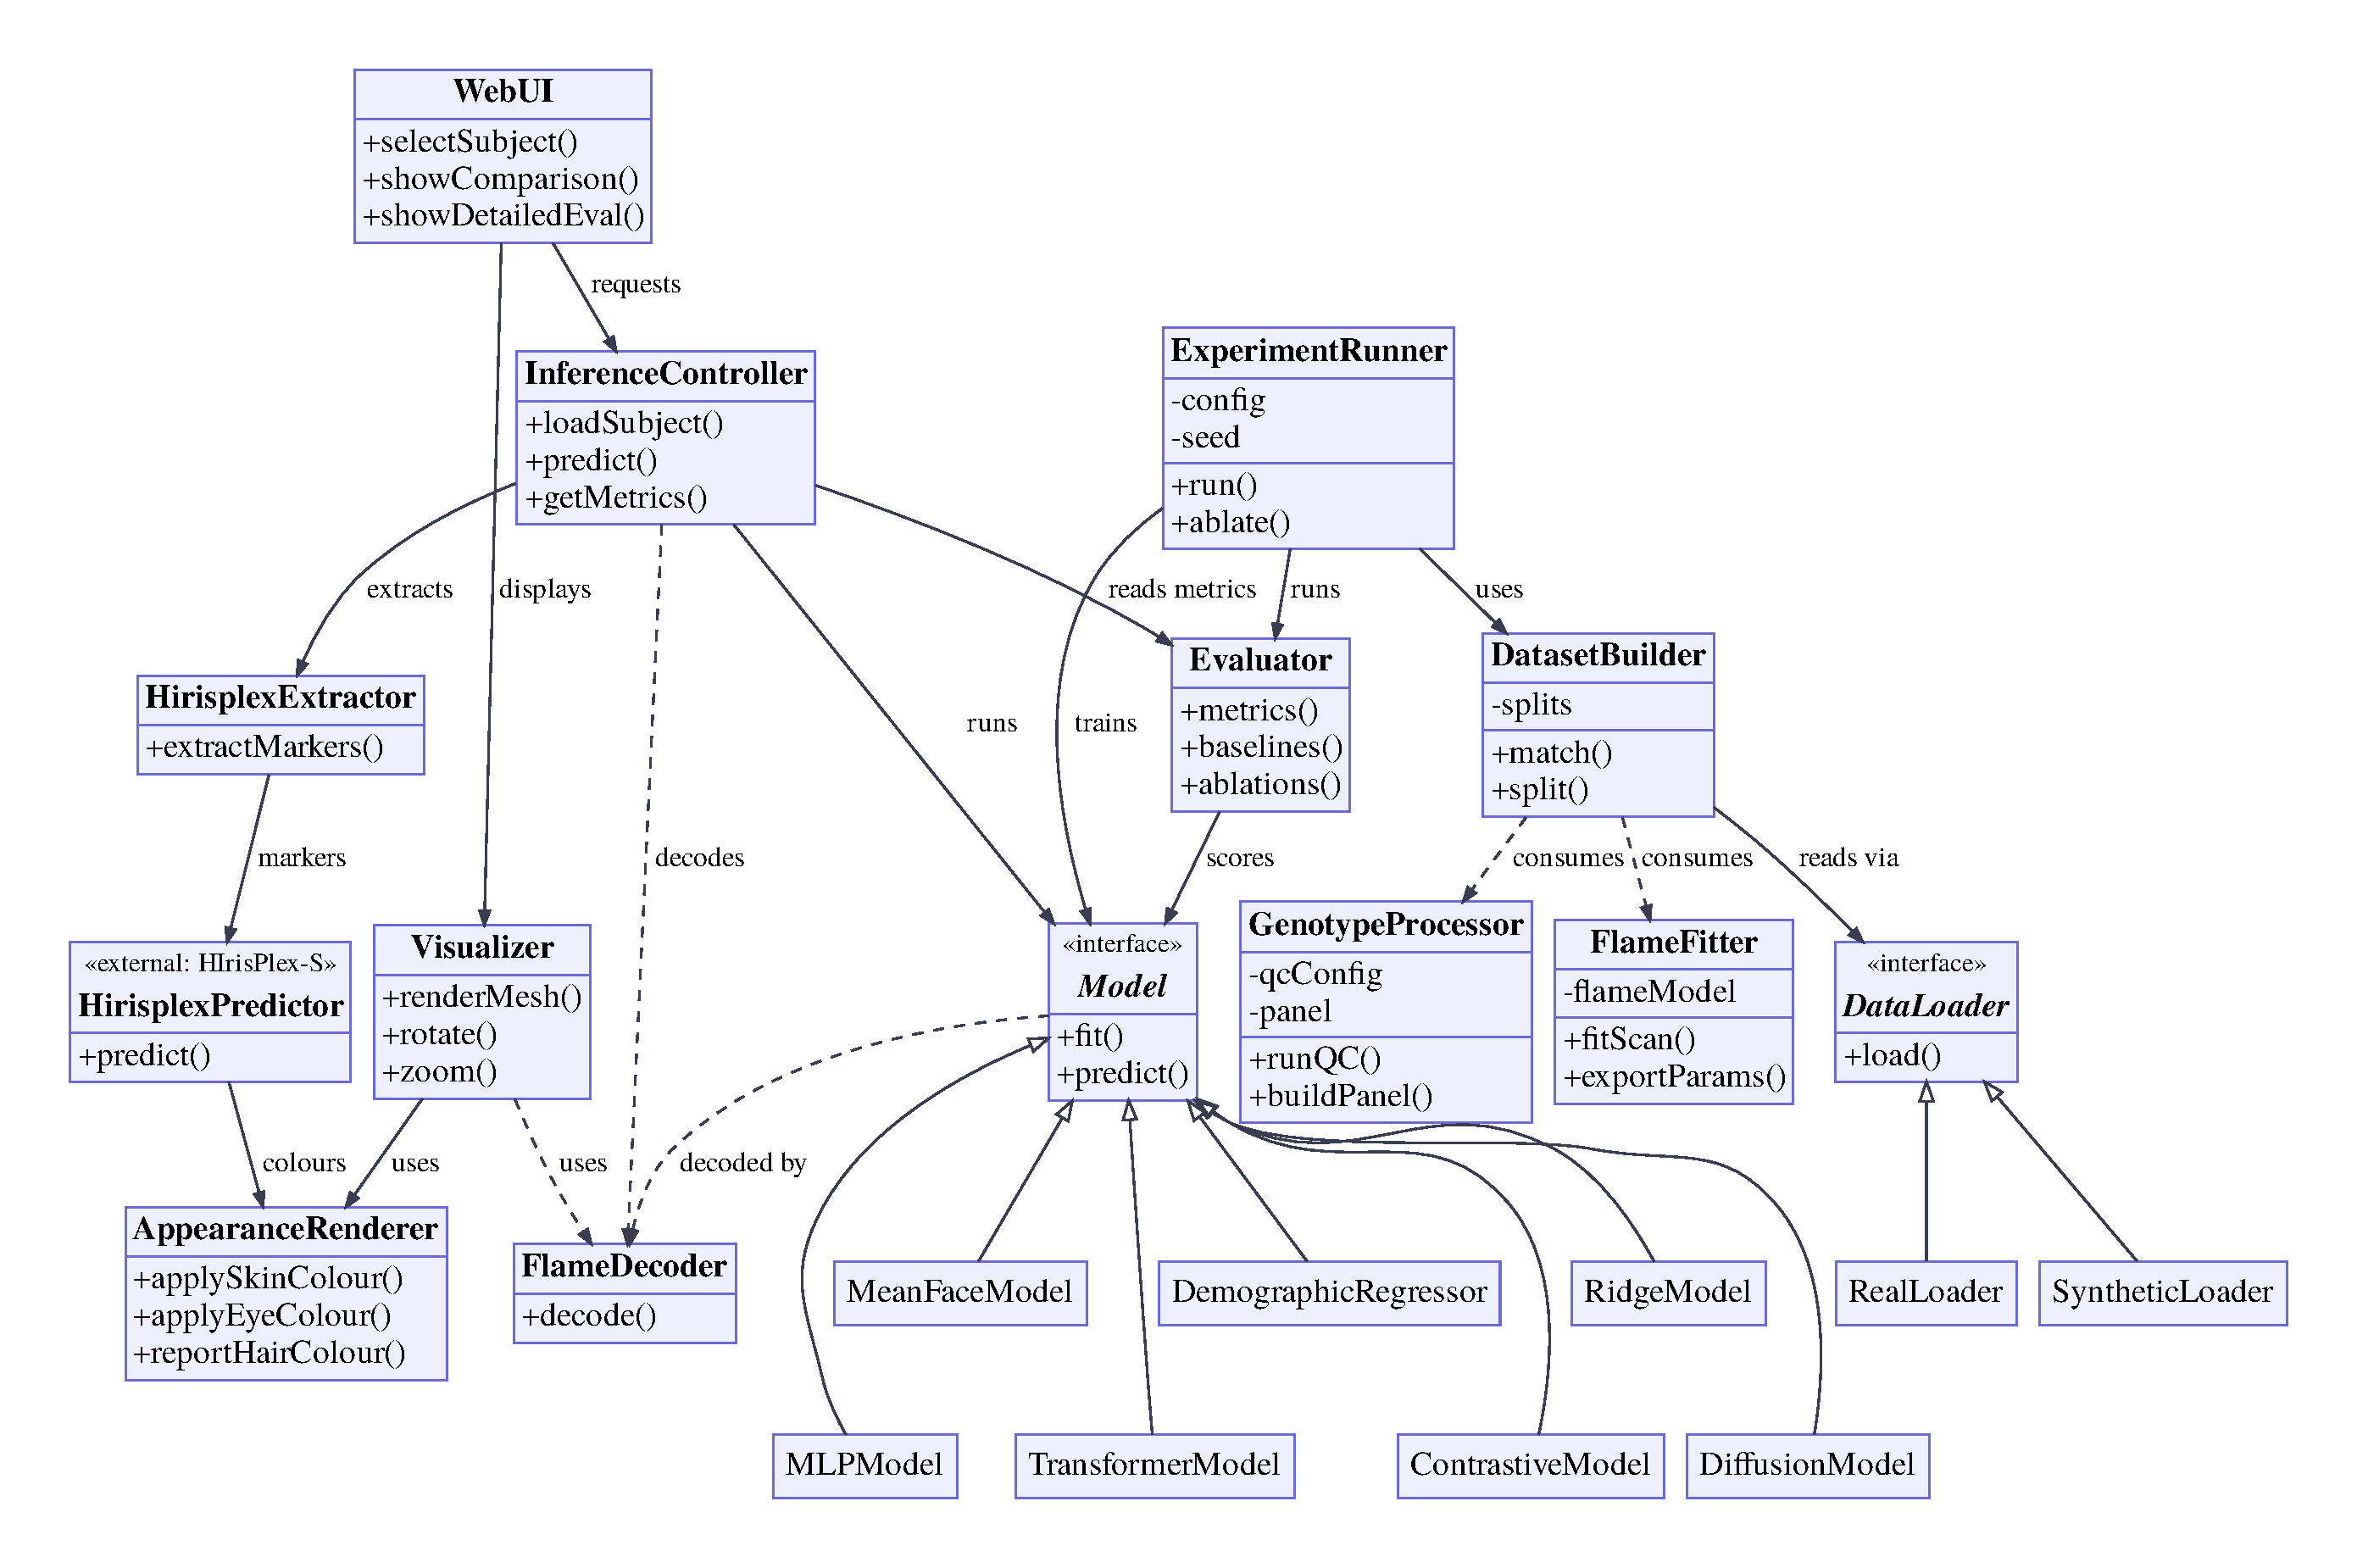
\includegraphics[width=0.98\textheight,height=0.86\textwidth,keepaspectratio]{Figures/class_diagram.pdf}
\caption{Class diagram of FaceCon.}
\label{fig:class}
\end{sidewaysfigure}

The diagram reflects the architecture directly. On the research side, \texttt{ExperimentRunner} is the orchestrator and is associated with \texttt{DatasetBuilder}, the \texttt{Model} interface, and \texttt{Evaluator}. \texttt{DatasetBuilder} depends on the outputs of \texttt{GenotypeProcessor} and \texttt{FlameFitter} and reads data through the \texttt{DataLoader} interface, which is realized by \texttt{SyntheticLoader} and \texttt{RealLoader} so that synthetic and real data are interchangeable. Every concrete predictor, from \texttt{MeanFaceModel} and \texttt{DemographicRegressor} through \texttt{RidgeModel}, \texttt{MLPModel}, and \texttt{TransformerModel}, realizes the single \texttt{Model} interface and is therefore interchangeable. Each model's predicted FLAME parameters are decoded by the shared \texttt{FlameDecoder}, and \texttt{Evaluator} computes metrics and baselines over the decoded meshes and the predicted parameters. The appearance component is a thin integration rather than a trained model: \texttt{HirisplexExtractor} selects the HIrisPlex-S marker SNPs from the same genotype, and \texttt{HirisplexPredictor} wraps the external, already-validated HIrisPlex-S method to return eye, hair, and skin colour; \texttt{AppearanceRenderer} then applies the predicted skin colour and eye colour to the decoded mesh and reports hair colour, rendering it only where suitable hair geometry exists. No appearance model is trained or scored by \texttt{Evaluator}. On the demonstrator side, \texttt{WebUI} requests predictions from \texttt{InferenceController}, which runs the trained \texttt{Model} and the integrated \texttt{HirisplexPredictor}, decodes the result through \texttt{FlameDecoder}, colours it through \texttt{AppearanceRenderer}, and reads metrics from \texttt{Evaluator}, while \texttt{Visualizer} renders the resulting faces in the interface. These demonstrator classes are the software counterparts of the interactions shown in the sequence diagrams of Section~\ref{sec:seq}.

\begin{table}[!ht]
\centering
\caption{Model inventory, all realizing the common Model interface and shared FLAME-decode contract.}
\label{tab:models}
\small
\begin{tabular}{|P{3.6cm}|P{3.2cm}|P{2.4cm}|P{3.0cm}|}
\hline
\textbf{Model} & \textbf{Input} & \textbf{Output} & \textbf{Role} \\ \hline
Mean face & --- & mean $Y_{\mathrm{face}}$ & Baseline 0 \\ \hline
Demographic regressor & $X_{\mathrm{demo}}$ & $Y_{\mathrm{face}}$ & Baseline 1 \\ \hline
Ridge & $X_{\mathrm{snp}}$ & $Y_{\mathrm{face}}$ & Baseline 2 \\ \hline
MLP & $X_{\mathrm{snp}}$ & $Y_{\mathrm{face}}$ & Baseline 3 \\ \hline
MLP & $X_{\mathrm{snp}} + X_{\mathrm{demo}}$ & $Y_{\mathrm{face}}$ & Baseline 4 \\ \hline
MLP / Ridge & GWAS SNP subset & $Y_{\mathrm{face}}$ & Baseline 5 \\ \hline
Same model & matched random SNPs & $Y_{\mathrm{face}}$ & Baseline 6 \\ \hline
Transformer SNP encoder & $X_{\mathrm{snp}}$ & latent / $Y_{\mathrm{face}}$ & Advanced \\ \hline
Contrastive SNP--face & SNP + face embeddings & aligned latents & Advanced (Stage 1) \\ \hline
Generative prior & SNP embedding & face embedding / shape & Advanced (Stage 2) \\ \hline
FLAME decoder & shape (+ expr/pose) & mesh vertices & Shared decode \\ \hline
\end{tabular}
\end{table}

The table lists only the trained shape models, which are what the \texttt{Model} interface makes interchangeable. The appearance colours are not a trained model and so do not appear in this inventory: they are produced by integrating the external HIrisPlex-S predictor, which takes the HIrisPlex-S marker SNPs extracted from the same genotype and returns eye, hair, and skin colour. HIrisPlex-S is used as published and is not scored against baselines, because the 3DFN resource does not provide eye, hair, or skin colour labels.

\section{Sequence Diagrams}
\label{sec:seq}
The sequence diagrams below describe the core demonstrator interactions and are consistent with the use cases of Section~\ref{sec:usecases}, the class diagram of Figure~\ref{fig:class}, and the layered architecture of Figure~\ref{fig:arch}. They involve the user, the web UI, the inference controller, the trained FaceCon model, the demographic baseline, the FLAME decoder, the evaluation module, and the 3D viewer, together with the preprocessed test data.

Figure~\ref{fig:seq1} shows the main workflow, in which a user selects a held-out test subject (UC-04), the system generates a prediction (UC-03), and the result is shown in the prediction view (UC-05). The inference controller loads the subject's preprocessed features, obtains the predicted FLAME parameters from the model, decodes the predicted and ground truth faces through the FLAME decoder, reads the metrics from the evaluation module, and returns them for the viewer to render.

\begin{sidewaysfigure}
\centering\setstretch{1}
\begin{tikzpicture}[font=\small,>=Latex]
\draw[seqline] (0.5,-0.62)--(0.5,-13.61);
\draw[thick,draw=seqc,fill=seqf] (0.5,0.22) circle (0.19);\draw[thick,draw=seqc] (0.5,0.03)--(0.5,-0.34) (0.22999999999999998,-0.1)--(0.77,-0.1) (0.5,-0.34)--(0.28,-0.62) (0.5,-0.34)--(0.72,-0.62);
\node[anchor=south] at (0.5,0.42) {User};
\draw[seqline] (4.4,-0.45)--(4.4,-13.61);
\node[seqbox] at (4.4,0) {Web UI};
\draw[seqline] (7.8,-0.45)--(7.8,-13.61);
\node[seqbox] at (7.8,0) {Inference\\Controller};
\draw[seqline] (13.4,-0.45)--(13.4,-13.61);
\node[seqbox] at (13.4,0) {Preprocessed\\Test Data};
\draw[seqline] (15.9,-0.45)--(15.9,-13.61);
\node[seqbox] at (15.9,0) {FaceCon\\Model};
\draw[seqline] (18.4,-0.45)--(18.4,-13.61);
\node[seqbox] at (18.4,0) {FLAME\\Decoder};
\draw[seqline] (20.9,-0.45)--(20.9,-13.61);
\node[seqbox] at (20.9,0) {Evaluation\\Module};
\draw[seqline] (23.3,-0.45)--(23.3,-13.61);
\node[seqbox] at (23.3,0) {3D Viewer};
\draw[seqcall] (0.5,-1.50)--(4.4,-1.50);
\draw[seqcall] (4.4,-2.29)--(7.8,-2.29);
\draw[seqcall] (7.8,-3.38)--(13.4,-3.38);
\draw[seqret] (13.4,-4.17)--(7.8,-4.17);
\draw[seqcall] (0.5,-5.26)--(4.4,-5.26);
\draw[seqcall] (4.4,-6.05)--(7.8,-6.05);
\draw[seqcall] (7.8,-6.84)--(15.9,-6.84);
\draw[seqret] (15.9,-7.63)--(7.8,-7.63);
\draw[seqcall] (7.8,-8.42)--(18.4,-8.42);
\draw[seqret] (18.4,-9.21)--(7.8,-9.21);
\draw[seqcall] (7.8,-10.00)--(20.9,-10.00);
\draw[seqret] (20.9,-10.79)--(7.8,-10.79);
\draw[seqret] (7.8,-11.58)--(4.4,-11.58);
\draw[seqcall] (4.4,-12.37)--(23.3,-12.37);
\draw[seqret] (23.3,-13.16)--(0.5,-13.16);
\node[seqlab] at (2.45,-1.44) {Select held-out\\test subject (UC-04)};
\node[seqlab] at (6.10,-2.23) {loadSubject(id)};
\node[seqlab] at (10.60,-3.32) {fetch SNP features, demographics,\\ground-truth FLAME};
\node[seqlab] at (10.60,-4.11) {features, demographics, ground truth};
\node[seqlab] at (2.45,-5.20) {Click ``Generate\\prediction'' (UC-04)};
\node[seqlab] at (6.10,-5.99) {predict(subject)};
\node[seqlab] at (11.85,-6.78) {predict(X\_snp, X\_demo)};
\node[seqlab] at (11.85,-7.57) {predicted FLAME parameters};
\node[seqlab] at (13.10,-8.36) {decode(prediction, ground truth)};
\node[seqlab] at (13.10,-9.15) {predicted and ground-truth meshes};
\node[seqlab] at (14.35,-9.94) {metrics(prediction, ground truth)};
\node[seqlab] at (14.35,-10.73) {mesh error, landmark error};
\node[seqlab] at (6.10,-11.52) {meshes and metrics};
\node[seqlab] at (13.85,-12.31) {render predicted mesh and comparison};
\node[seqlab] at (11.90,-13.10) {Prediction screen (UC-05)};
\node[seqnum] at (0.5,-1.50) {1};
\node[seqnum] at (4.4,-2.29) {2};
\node[seqnum] at (7.8,-3.38) {3};
\node[seqnum] at (13.4,-4.17) {4};
\node[seqnum] at (0.5,-5.26) {5};
\node[seqnum] at (4.4,-6.05) {6};
\node[seqnum] at (7.8,-6.84) {7};
\node[seqnum] at (15.9,-7.63) {8};
\node[seqnum] at (7.8,-8.42) {9};
\node[seqnum] at (18.4,-9.21) {10};
\node[seqnum] at (7.8,-10.00) {11};
\node[seqnum] at (20.9,-10.79) {12};
\node[seqnum] at (7.8,-11.58) {13};
\node[seqnum] at (4.4,-12.37) {14};
\node[seqnum] at (23.3,-13.16) {15};
\end{tikzpicture}

\caption{Sequence diagram for prediction generation (UC-04, UC-03, UC-05).}
\label{fig:seq1}
\end{sidewaysfigure}

Figure~\ref{fig:seq2} shows the evaluation and results interaction (UC-06), in which the inference controller requests the demographic baseline shape, the regional errors, and the summary metrics from the evaluation module and returns them for display.

\begin{sidewaysfigure}
\centering\setstretch{1}
\begin{tikzpicture}[font=\small,>=Latex]
\draw[seqline] (0.5,-0.62)--(0.5,-12.05);
\draw[thick,draw=seqc,fill=seqf] (0.5,0.22) circle (0.19);\draw[thick,draw=seqc] (0.5,0.03)--(0.5,-0.34) (0.22999999999999998,-0.1)--(0.77,-0.1) (0.5,-0.34)--(0.28,-0.62) (0.5,-0.34)--(0.72,-0.62);
\node[anchor=south] at (0.5,0.42) {User};
\draw[seqline] (5.2,-0.45)--(5.2,-12.05);
\node[seqbox] at (5.2,0) {Web UI};
\draw[seqline] (10.2,-0.45)--(10.2,-12.05);
\node[seqbox] at (10.2,0) {Inference\\Controller};
\draw[seqline] (15.4,-0.45)--(15.4,-12.05);
\node[seqbox] at (15.4,0) {Demographic\\Baseline};
\draw[seqline] (19.4,-0.45)--(19.4,-12.05);
\node[seqbox] at (19.4,0) {Evaluation\\Module};
\draw[seqline] (23.0,-0.45)--(23.0,-12.05);
\node[seqbox] at (23.0,0) {3D Viewer};
\draw[seqcall] (0.5,-1.50)--(5.2,-1.50);
\draw[seqcall] (5.2,-2.45)--(10.2,-2.45);
\draw[seqcall] (10.2,-3.40)--(15.4,-3.40);
\draw[seqret] (15.4,-4.65)--(10.2,-4.65);
\draw[seqcall] (10.2,-5.60)--(19.4,-5.60);
\draw[seqret] (19.4,-6.55)--(10.2,-6.55);
\draw[seqcall] (10.2,-7.50)--(19.4,-7.50);
\draw[seqret] (19.4,-8.45)--(10.2,-8.45);
\draw[seqret] (10.2,-9.70)--(5.2,-9.70);
\draw[seqcall] (5.2,-10.65)--(23.0,-10.65);
\draw[seqret] (23.0,-11.60)--(0.5,-11.60);
\node[seqlab] at (2.85,-1.44) {Open ``Evaluation and\\Results'' (UC-05)};
\node[seqlab] at (7.70,-2.39) {getEvaluation(subject)};
\node[seqlab] at (12.80,-3.34) {baselineShape(demographics)};
\node[seqlab] at (12.80,-4.59) {demographic-baseline\\FLAME parameters};
\node[seqlab] at (14.80,-5.54) {regionalErrors(prediction, ground truth)};
\node[seqlab] at (14.80,-6.49) {per-region errors (nose, jaw, eyes, mouth)};
\node[seqlab] at (14.80,-7.44) {summaryMetrics(baseline, prediction, ground truth)};
\node[seqlab] at (14.80,-8.39) {mean mesh error, landmark error, retrieval rank};
\node[seqlab] at (7.70,-9.64) {baseline, prediction,\\ground truth and metrics};
\node[seqlab] at (14.10,-10.59) {render three faces with error colouring};
\node[seqlab] at (11.75,-11.54) {Evaluation and Results screen (UC-06)};
\node[seqnum] at (0.5,-1.50) {1};
\node[seqnum] at (5.2,-2.45) {2};
\node[seqnum] at (10.2,-3.40) {3};
\node[seqnum] at (15.4,-4.65) {4};
\node[seqnum] at (10.2,-5.60) {5};
\node[seqnum] at (19.4,-6.55) {6};
\node[seqnum] at (10.2,-7.50) {7};
\node[seqnum] at (19.4,-8.45) {8};
\node[seqnum] at (10.2,-9.70) {9};
\node[seqnum] at (5.2,-10.65) {10};
\node[seqnum] at (23.0,-11.60) {11};
\end{tikzpicture}

\caption{Sequence diagram for evaluation and results (UC-06).}
\label{fig:seq2}
\end{sidewaysfigure}

Figure~\ref{fig:seq3} shows the simple return interaction, in which the user navigates from the evaluation and results view back to subject selection and the system resets the viewers and reloads the list of held-out subjects.

\begin{figure}[!ht]
\centering\setstretch{1}
% Figure 6.5: return to subject selection (UC-06, UC-04).
% Redrawn as vector graphics in the style of Figures 6.3 and 6.4; the earlier
% raster version used a different typeface and its self-call label crossed the lifeline.
\begin{tikzpicture}[font=\small,>=Latex]
\draw[seqline] (0.5,-0.62)--(0.5,-6.55);
\draw[thick,draw=seqc,fill=seqf] (0.5,0.22) circle (0.19);\draw[thick,draw=seqc] (0.5,0.03)--(0.5,-0.34) (0.23,-0.1)--(0.77,-0.1) (0.5,-0.34)--(0.28,-0.62) (0.5,-0.34)--(0.72,-0.62);
\node[anchor=south] at (0.5,0.42) {User};
\draw[seqline] (6.4,-0.45)--(6.4,-6.55);
\node[seqbox] at (6.4,0) {Web UI};
\draw[seqline] (12.6,-0.45)--(12.6,-6.55);
\node[seqbox] at (12.6,0) {Inference\\Controller};
% messages
\draw[seqcall] (0.5,-1.40)--(6.4,-1.40);
\draw[seqcall] (6.4,-2.35)--(7.5,-2.35)--(7.5,-2.95)--(6.4,-2.95);
\draw[seqcall] (6.4,-3.95)--(12.6,-3.95);
\draw[seqret] (12.6,-4.90)--(6.4,-4.90);
\draw[seqret] (6.4,-5.85)--(0.5,-5.85);
% labels
\node[seqlab] at (3.45,-1.34) {Click ``Back to subject\\selection'' (UC-06)};
\node[anchor=west,inner sep=1.5pt,align=left,font=\small] at (7.65,-2.65) {reset viewers and\\selection state};
\node[seqlab] at (9.50,-3.89) {listTestSubjects()};
\node[seqlab] at (9.50,-4.84) {available held-out subjects};
\node[seqlab] at (3.45,-5.79) {Test Subject Selection\\screen (UC-04)};
% step numbers
\node[seqnum] at (0.5,-1.40) {1};
\node[seqnum] at (6.4,-2.35) {2};
\node[seqnum] at (6.4,-3.95) {3};
\node[seqnum] at (12.6,-4.90) {4};
\node[seqnum] at (6.4,-5.85) {5};
\end{tikzpicture}

\caption{Sequence diagram for returning to subject selection (UC-06, UC-04).}
\label{fig:seq3}
\end{figure}

\section{Policies and Tactics}
This section records design policies and tactics that shape the implementation without altering the high-level architecture. Where the architecture fixes which components exist, these policies fix how they must behave, and most of them exist to protect the validity of the results. They cover the contracts between components, the handling of controlled-access data, reproducibility, the prevention of data leakage, input validation, and the traceability of tests to requirements.

\subsection{Interface Contracts}
\label{sec:interfaces}
The system is held together by six small, explicit interface contracts, which also make synthetic and real data interchangeable.
\begin{itemize}
\item The genotype interface produces $X_{\mathrm{snp}}$ and subject identifiers, and is interchangeable between synthetic and real data loaders.
\item The face interface produces $Y_{\mathrm{face}}$, and optionally a mesh and landmarks, from FLAME fitting.
\item The model interface is \texttt{predict(X\_snp, X\_demo=None) -> Y\_face\_hat}.
\item The decode interface is \texttt{flame\_decode(Y\_face\_hat) -> vertices, faces}.
\item The appearance interface is \texttt{hirisplex\_predict(X\_markers) -> eye, hair, skin colour}, wrapping the external HIrisPlex-S predictor over the extracted marker SNPs, plus a renderer that applies the predicted colours to the decoded mesh.
\item The evaluation interface compares shape predictions and meshes against held-out targets and baselines.
\end{itemize}

\subsection{Data Handling, Privacy, and Access Control}
Raw genotype and scan data are used only under the approved data-use agreement and are never written into released code, figures, or the demonstrator. Raw and processed data are kept in separate locations, and only de-identified, processed artifacts cross into the modelling and demonstration stages. The demonstrator operates on preprocessed test data and never exposes raw genotype information.

\subsection{Reproducibility and Experiment Consistency}
Every run is driven by a configuration file and a fixed random seed, dependencies are pinned, and per-run configurations are captured. All models are evaluated on identical data splits and with the same metric implementations, so that comparisons across the baselines first progression are consistent.

\subsection{Data-Leakage Prevention and Model Selection}
Splits are strictly subject-level and respect relatedness. Any dataset-derived statistics, such as normalization parameters or within-dataset SNP selection, are fitted on the training folds only. Model selection uses the validation split, and the test split is reserved for final reporting.

\subsection{Input Validation and Error Handling}
Each module validates its inputs and fails safely on malformed data, reporting the error and halting rather than producing invalid output. Missing SNPs at inference are imputed or masked according to the documented policy, and subjects that cannot be fitted to FLAME within the error threshold are flagged and excluded with a recorded reason.

\subsection{Coding, Testing, and Traceability}
Coding conventions require modular packages per pipeline stage, typed function signatures, and no hard-coded machine-specific paths. Each module is unit-tested on synthetic inputs, and an end-to-end integration test runs on synthetic data before real data is used. Requirements traceability is maintained by linking each functional requirement to a use case and a planned test.

\section{Conclusion}
This chapter has presented FaceCon's design as a four-layer modular architecture. The interface layer, the processing layer, the model layer, and the data layer each have one responsibility, and they communicate only through the small set of explicit contracts recorded in this chapter. Several architectural strategies were considered, and a layered pipeline with interchangeable models behind a shared interface was selected because it lets the simplest baseline and the most complex network be trained, evaluated, and compared through exactly the same code. The class diagram makes that structure precise, distinguishing the associations, dependencies, and inheritance between the components, and the sequence diagrams show how the main use cases move through them at run time. The policies and tactics turn the requirements of Chapter~\ref{ch:srs} into rules the code must follow, covering privacy and access control, reproducibility, the prevention of data leakage, input validation, and the traceability of tests to requirements. The next chapter describes the prototype that implements this design and the test cases that verify it.
